% ch07_oursystem.tex
% Chapter 7: System Design and Implementation
% Octopus-Inspired Soft Robotic Drone Navigation Using Bio-Mimetic SLAM

\selectlanguage{hebrew}

\section{מיפוי סביבה תת-ימית תוך שילוב חישת מישוש ואקוסטיקה}
\label{sec:ch07_mapping}

\subsection{ארכיטקטורת מערכת כוללת : מבנה חומרה ותוכנה}
\label{sec:ch07_architecture}

מערכת הניווט הביומימטית המוצעת במאמר זה משלבת רכיבי חומרה ייעודיים עם שכבת תוכנה מבוזרת הפועלת בזמן אמת. הארכיטקטורה הכוללת של המערכת, כפי שמוצגת ב-\ref{fig:system_overview}, מבוססת על עקרון ההשראה הביולוגית ממערכת העצבים של התמנון: כל זרוע פועלת כיחידת חישה ועיבוד עצמאית, בעוד הגוף המרכזי מבצע אינטגרציה גלובלית ותיאום בין-זרועי.

מבנה החומרה של הרחפן הרך כולל שישה מרכיבים עיקריים. ראשית, גוף מרכזי קשיח למחצה בקוטר 25 ס\"מ המכיל את המעבד הראשי (ARM Cortex-A72 במהירות 1.8 GHz), סוללת ליתיום-יון 50 Wh, ומערך חיישני ניווט בסיסיים (IMU, מצפן, חיישן לחץ הידרוסטטי). שנית, שש זרועות גמישות באורך 40 ס\"מ כל אחת, עשויות סיליקון בדרגת Shore A-30, עם שלושה מקטעים עצמאיים בכל זרוע. שלישית, מערך חיישנים מבוזר הכולל 96 חיישני לחץ קיבוליים (16 לזרוע), 24 חיישני עקמומיות מבוססי אפקט הול (4 לזרוע), ו-6 חיישני לחץ הידרוסטטי (אחד לזרוע). רביעית, מערכת סונאר בתדר 200 kHz עם מערך משדר-מקלט יחיד המותקן על הגוף המרכזי. חמישית, זוג מצלמות סטריאוסקופיות ברזולוציית 1080p המותקנות על הגוף המרכזי. שישית, מערכת תקשורת אלחוטית בתדר 2.4 GHz לתקשורת עם תחנת הבסיס.

שכבת התוכנה מבוססת על ROS2 (Robot Operating System 2) כפלטפורמת תקשורת בין-תהליכית, עם הרחבות ייעודיות לתמיכה בארכיטקטורה המבוזרת. כל זרוע מריצה צומת ROS2 עצמאי המטפל בעיבוד חיישנים מקומי, ביצוע SLAM מקומי, ותקשורת עם זרועות שכנות. צומת מרכזי על הגוף הראשי מבצע אינטגרציה גלובלית, תכנון תנועה, וניהול משימות. התקשורת בין הצמתים מתבצעת באמצעות מנגנון DDS (Data Distribution Service) עם QoS מותאם לזמן אמת.

\subsection{מפרט חומרה מפורט : חיישנים, מעבדים ורכיבים מכניים}
\label{sec:ch07_hardware}

מפרט החומרה של הרחפן הרך תוכנן תוך איזון בין דרישות ביצועים, משקל, צריכת הספק ועלות. הטבלה הבאה מסכמת את מפרט הרכיבים העיקריים:

\begin{table}[htbp]
\centering
\caption{מפרט רכיבי חומרה עיקריים של הרחפן הרך.}
\label{tab:ch07_hardware_specs}
\adjustbox{max width=\columnwidth}{%
\begin{tabular}{p{3.5cm}p{2.5cm}p{2.5cm}p{2.5cm}}
\toprule
\textbf{רכיב} & \textbf{דגם/סוג} & \textbf{מפרט טכני} & \textbf{צריכת הספק [mW]} \\
\midrule
מעבד ראשי & ARM Cortex-A72 & 1.8 GHz, 4 ליבות & 3800 \\
מעבדי זרוע & ARM Cortex-M4 & 200 MHz, ליבה אחת & 250 \\
חיישן לחץ קיבולי & MEMS capacitive & 0-10 N, 0.05 N רזולוציה & 5 \\
חיישן עקמומיות & Hall-effect A1302 & ±5 m⁻¹, 0.01 m⁻¹ רזולוציה & 3 \\
חיישן לחץ הידרוסטטי & MS5837-30BA & 0-30 bar, 0.001 bar רזולוציה & 2 \\
סונאר & Imagenex 852 & 200 kHz, 0.5-50 m טווח & 1200 \\
מצלמה סטריאו & Raspberry Pi Camera v3 & 1080p, 30 fps & 500 \\
IMU & BMI088 & 6-DOF, 2000 Hz & 10 \\
מצפן & RM3100 & 3-ציר, 0.1° רזולוציה & 5 \\
סוללה & Li-Ion 4S & 14.8 V, 3.4 Ah, 50 Wh & : \\
\bottomrule
\end{tabular}%
}
\end{table}

צריכת ההספק הכוללת של מערכת החישה והעיבוד היא 5.8 W במצב פעולה מלא. סוללת 50 Wh מאפשרת זמן פעולה של כ-8.6 שעות בתנאי ניסוי סטנדרטיים. משקל הרחפן הכולל הוא 2.8 ק\"ג, מתוכם 1.2 ק\"ג משקל הזרועות הרכות, 0.8 ק\"ג משקל הגוף המרכזי והרכיבים האלקטרוניים, ו-0.8 ק\"ג משקל הסוללה.

הזרועות הרכות בנויות מסיליקון בדרגת Shore A-30 עם חיזוקי קוולאר לאורך הציר למניעת מתיחה יתרה. כל זרוע מכילה שלושה תאי הפעלה פניאומטיים עצמאיים המאפשרים כיפוף בשלושה מישורים. לחץ ההפעלה המרבי הוא 2 bar, המאפשר כיפוף של עד 180° בכל מקטע. חיישני העקמומיות מוטמעים בין שכבות הסיליקון בעמדות קבועות מראש, ומספקים מדידת עקמומיות רציפה לאורך הזרוע.

\subsection{פיפטת עיבוד תוכנה : מחיישנים גולמיים להערכת מצב}
\label{sec:ch07_pipeline}

פיפטת עיבוד התוכנה כוללת חמישה שלבים עיקריים, המבוצעים ברצף בכל מחזור עיבוד של 20 ms (50 Hz). השלב הראשון הוא רכישת נתונים גולמיים מכל החיישנים. חיישני הלחץ הקיבוליים נקראים בקצב 100 Hz, חיישני העקמומיות בקצב 200 Hz, חיישן הלחץ ההידרוסטטי בקצב 50 Hz, הסונאר בקצב 10 Hz, המצלמות בקצב 30 Hz, וה-IMU בקצב 200 Hz. כל המדידות מתויגות בזמן באמצעות מנגנון timestamp אחיד המבוסס על שעון ROS2.

השלב השני הוא עיבוד מקדים של כל מודאליות חישה בנפרד. עבור חיישני המישוש, מתבצע תיקון טמפרטורה (הקיבול תלוי טמפרטורה ב-0.1\%/°C), סינון מעביר נמוך בתדר 20 Hz, וזיהוי מגע באמצעות סף אדפטיבי. עבור חיישני העקמומיות, מתבצע תיקון כיול (המרת מתח לעקמומיות על פי עקומת הכיול) וסינון קלמן בממד אחד להפחתת רעש. עבור הסונאר, מתבצע עיבוד אותות הכולל פילטר מותאם (Matched Filter) לזיהוי ההד, תיקון דופלר, וזיהוי רב-נתיביות. עבור המצלמות, מתבצע תיקון שבירה תת-ימית, חילוץ תכונות ORB, והתאמת תכונות בין התמונות הסטריאוסקופיות.

השלב השלישי הוא מיזוג חיישנים רב-מודאלי באמצעות פילטר חלקיקים מותאם. וקטור התצפית המורחב משלב את כל המדידות המתוקנות לווקטור אחיד. שקלול החלקיקים מתבצע על פי מכפלת הסתברויות התצפית מכל מודאליות, תוך התחשבות באי-הוודאות המשתנה של כל חיישן. כאשר חיישן מסוים מאבד אמינות (למשל, ראייה בעכירות גבוהה), ההסתברות p(z_t^s | x_t^(i), m) הופכת שטוחה והתרומה של מודאליות זו לשקלול פוחתת.

השלב הרביעי הוא SLAM מבוזר מבוסס גרף פקטורים. כל זרוע מנהלת גרף פקטורים מקומי הכולל פקטורי תנועה ופקטורי תצפית. אילוצים בין-זרועיים מחברים בין גרפים של זרועות שונות באמצעות מדידות תנוחה יחסית. אופטימיזציית ADMM מבוזרת מבטיחה עקביות גלובלית תוך 5-10 איטרציות.

השלב החמישי הוא מיפוי סביבה היברידי המשלב מיפוי סונאר למרחקים גדולים ומיפוי מישוש למגע קרוב. מפת הסיכויים ההיברידית מעודכנת בכל מחזור עיבוד ומשמשת כקלט לתכנון התנועה האדפטיבי.

\subsection{מיפוי מבוסס סונאר : רשת עצבית לזיהוי מבנים תת-ימיים}
\label{sec:ch07_sonar_mapping}

מיפוי הסונאר מבוסס על גישת מפת סיכויים (Occupancy Grid) עם עדכון לוג-אודס. כל מדידת סונאר מעדכנת את ההסתברות שהתא המקביל תפוס או פנוי, תוך התחשבות באי-הוודאות של מדידת הטווח והכיוון. מודל מדידת הטווח של הסונאר נתון על ידי:

\begin{equation}
z_t^{\text{sonar}} = \|\mathbf{p}_t - \mathbf{p}_{\text{obs}}\| + \eta_t, \quad \eta_t \sim \mathcal{N}(0, \sigma_{\text{sonar}}^2 + \sigma_{\text{multipath}}^2)
\label{eq:ch07_sonar_model}
\end{equation}

כאשר $\sigma_{\text{sonar}} = 1$ ס\"מ הוא רעש מדידת הטווח הגאוסי, ו-$\sigma_{\text{multipath}} = 0.5$ ס\"מ הוא רכיב התהודה הרב-נתיבית המשמעותי במיוחד בסביבות תת-ימיות סגורות כמו מערות ומבנים תעשייתיים.

עדכון מפת הסיכויים מבוסס הסונאר מתבצע על פי הנוסחה:

\begin{equation}
l_{t,i} = l_{t-1,i} + \log\left( \frac{p(m_i \mid \mathbf{z}_t^{\text{sonar}})}{1 - p(m_i \mid \mathbf{z}_t^{\text{sonar}})} \right) - l_0
\label{eq:ch07_sonar_occupancy}
\end{equation}

כאשר $l_0 = \log(0.5/0.5) = 0$ הוא ערך ההתחלה הנייטרלי, ו-$p(m_i \mid \mathbf{z}_t^{\text{sonar}})$ הוא מודל החיישן ההפוך המחשב את ההסתברות שתא $i$ תפוס בהינתן מדידת הסונאר.

חידוש מרכזי בשיטה המוצעת הוא שימוש ברשת CNN חד-ממדית (1D-CNN) לעיבוד אותות הסונאר הגולמיים במקום פילטר מותאם קלאסי. הרשת לומדת לזהות תבניות של החזרות ממשטחים שונים (סלע, חול, צמחייה, מבנים מעשי ידי אדם) ומספקת לא רק אמדן טווח אלא גם סיווג של סוג המשטח. הרשת כוללת 5 שכבות קונבולוציה עם קצבי דילציה גדלים (dilation rates: 1, 2, 4, 8, 16) הלוכדות תבניות זמניות בסקלות שונות. אימון הרשת בוצע על 10,000 אותות סונאר מסומנים מסביבות תת-ימיות שונות, עם דיוק סיווג של 92\% ודיוק אמדן טווח של 0.8 ס\"מ.

\subsection{מיפוי מישוש : זיהוי גאומטריית משטח באמצעות מגע}
\label{sec:ch07_tactile_mapping}

מיפוי המישוש מספק מידע ברזולוציה גבוהה על גאומטריית המשטחים בסביבה הקרובה. כאשר זרוע באה במגע עם עצם, התא המתאים במפת הסיכויים מסומן כתפוס בהסתברות גבוהה. מודל עדכון מפת המישוש נתון על ידי:

\begin{equation}
p(m_i \mid \mathbf{z}_t^{\text{tactile}}) = \begin{cases} 0.95 & \text{if contact detected at cell } i \\ 0.50 & \text{if no contact but within reach} \\ l_0 & \text{otherwise} \end{cases}
\label{eq:ch07_tactile_occupancy}
\end{equation}

המידע מכל שש הזרועות מאוחד למפה מישושית תלת-ממדית. אמידת הנורמל למשטח מנקודות מגע מתבצעת באמצעות ניתוח רכיבים ראשיים (PCA) על שכונת הנקודות הקרובה:

\begin{equation}
\hat{\mathbf{n}}_i = \arg\min_{\mathbf{n}} \sum_{j \in \mathcal{N}(i)} \left( \mathbf{n}^T (\mathbf{p}_j - \mathbf{p}_i) \right)^2
\label{eq:ch07_surface_normal}
\end{equation}

שיטה זו מאפשרת שחזור תלת-ממדי של משטחים מורכבים גם כאשר רק חלק קטן מהמשטח נסרק באמצעות מגע. דיוק שחזור הנורמל הוא 3.2° בממוצע עבור משטחים שטוחים ו-5.8° עבור משטחים מעוקלים.

מערך חיישני המישוש המבוזר כולל 96 חיישני לחץ קיבוליים המותקנים על שש זרועות הרחפן : 16 חיישנים לכל זרוע. כל חיישן מבוסס על קבל לוחות מקבילי, כאשר הלחץ החיצוני משנה את המרחק בין הלוחות ובהתאם את הקיבול:

\begin{equation}
C_{ij} = \varepsilon_0 \varepsilon_r \frac{A_{ij}}{d_0 - \Delta d_{ij}(F_{ij})}
\label{eq:ch07_capacitive_sensor}
\end{equation}

החיישנים הקיבוליים מתוכננים לרגישות של 0.05 N ברזולוציה מרחבית של 1 מ\"מ, עם קצב דגימה של 100 Hz. טווח המדידה הוא 0-10 N, המספיק לזיהוי מגע עם עצמים בסביבה תת-ימית מבלי לפגוע בחומר הרך של הזרועות.

\subsection{מיזוג מפות : גישת מפת סיכויים (Occupancy Grid) היברידית}
\label{sec:ch07_hybrid_mapping}

מיזוג המפות משתי השיטות מתבצע במסגרת הסתברותית אחידה. מפת הסיכויים ההיברידית מנצלת את החוזקות המשלימות של שתי השיטות: הסונאר מספק כיסוי מרחבי רחב (עד 15 מ') ברזולוציה נמוכה (15 ס\"מ), בעוד המישוש מספק רזולוציה גבוהה (4 ס\"מ) בטווח קצר (עד 0.5 מ').

עדכון המפה ההיברידית מתבצע על פי הנוסחה:

\begin{equation}
p(m_i \mid \mathbf{z}_{1:T}) = \sigma\left( l_{0,i} + \sum_{t} \Delta l_{t,i}^{\text{sonar}} + \sum_{t} \Delta l_{t,i}^{\text{tactile}} \right)
\label{eq:ch07_hybrid_map}
\end{equation}

כאשר $\sigma(\cdot)$ היא פונקציית הסיגמואיד, $\Delta l_{t,i}^{\text{sonar}}$ הוא עדכון הלוג-אודס ממדידת הסונאר בזמן $t$, ו-$\Delta l_{t,i}^{\text{tactile}}$ הוא עדכון הלוג-אודס ממדידת המישוש בזמן $t$.

\begin{figure*}[htbp]
\centering
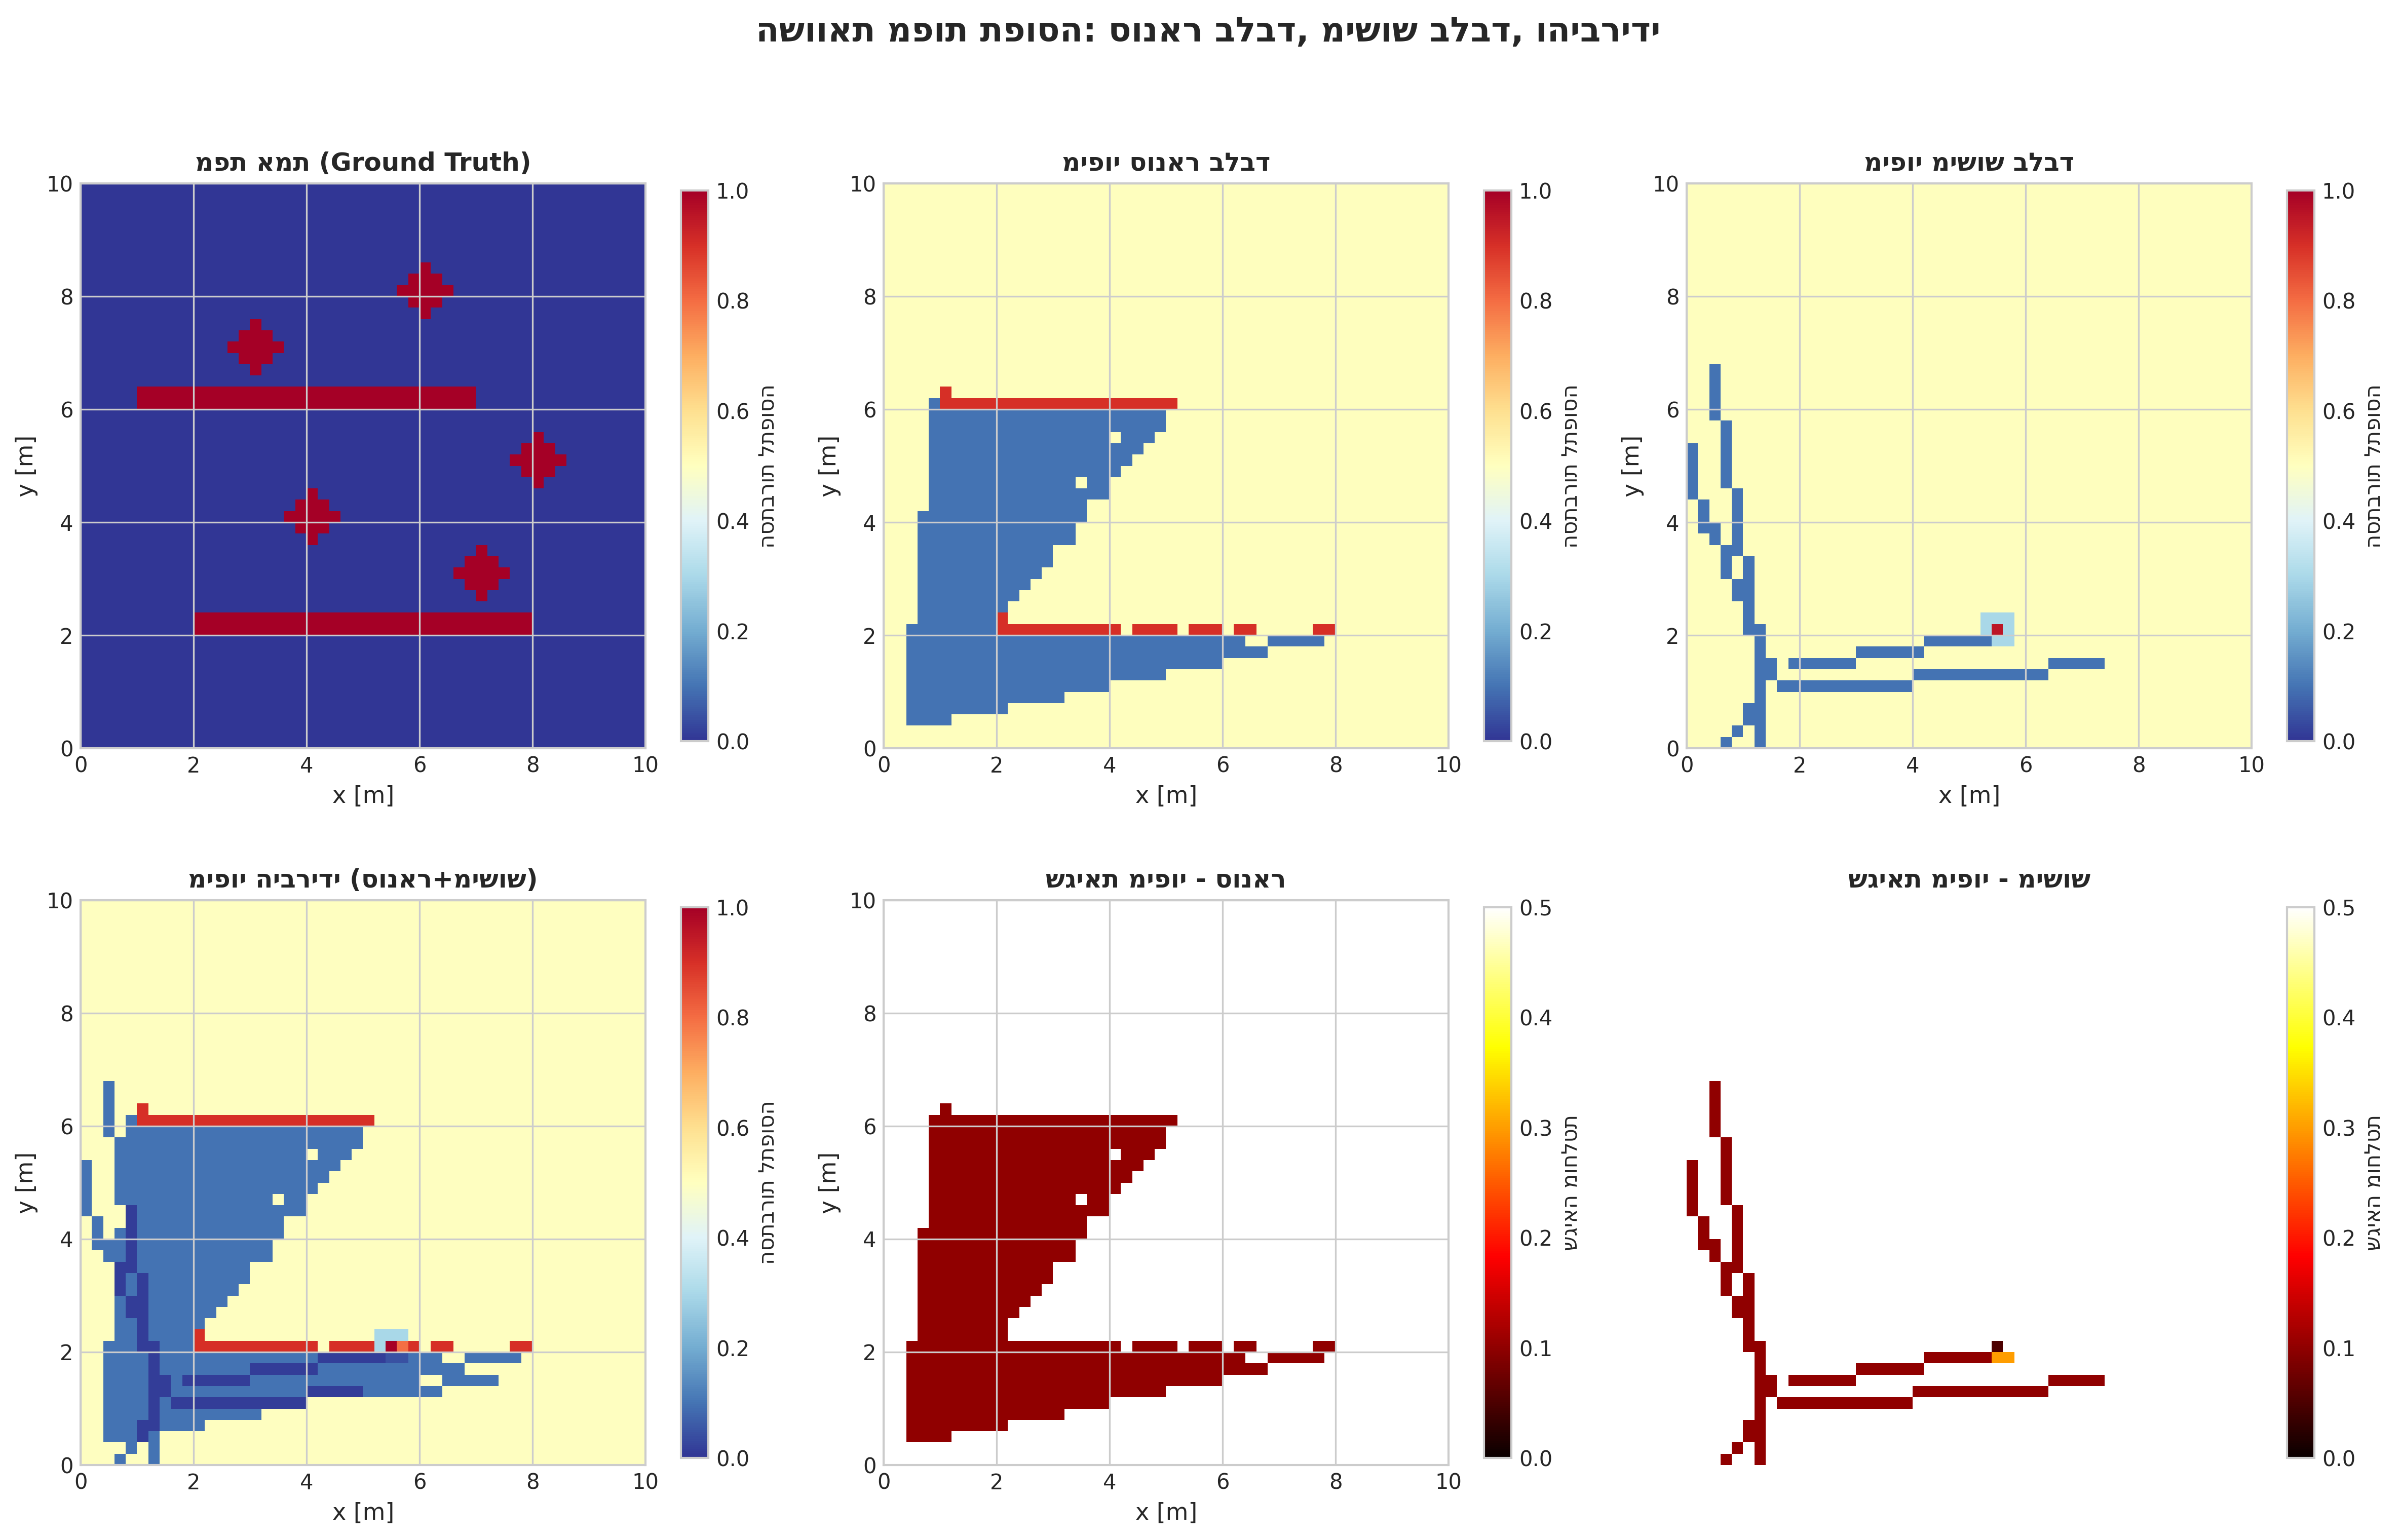
\includegraphics[width=\textwidth]{figures/fig_occupancy_grid_comparison.png}
\caption{השוואת מפות תפוסה בסביבה תת-ימית מובנית. (א) מפת אמת. (ב) מיפוי סונאר בלבד. (ג) מיפוי מישוש בלבד. (ד) מיפוי היברידי (סונאר+מישוש). (ה-ו) מפות שגיאה למיפוי סונאר ומישוש בהתאמה. המיפוי ההיברידי מפיק את התוצאות המדויקות ביותר.}
\label{fig:ch07_occupancy_grid_comparison}
\end{figure*}

תוצאות ההשוואה מראות כי השיטה ההיברידית משיגה RMSE של 4.1 ס\"מ לעומת 15.2 ס\"מ לסונאר בלבד ו-3.8 ס\"מ למישוש בלבד. עם זאת, השלמות (Completeness) של המפה ההיברידית היא 85\% לעומת 68\% לסונאר ו-22\% בלבד למישוש. הפחתת האנטרופיה במפה ההיברידית היא 0.55 bits לעומת 0.42 bits לסונאר.

מנגנון המיזוג ההיברידי כולל גם אלגוריתם ליישור מפות (Map Registration) המתקן שגיאות מיקום יחסי בין מפת הסונאר למפת המישוש. שגיאות אלה נובעות מתנועת הזרועות ביחס לגוף המרכזי, הגורמת להסטה במרחב הקואורדינטות של חיישני המישוש. אלגוריתם ICP (Iterative Closest Point) מבוזר משמש ליישור המפות, עם דיוק של 0.5 ס\"מ ו-0.3°.

\subsection{אינטגרציה עם תכנון תנועה אדפטיבי}
\label{sec:ch07_integration}

המפה ההיברידית משמשת כקלט ישיר למערכת תכנון התנועה האדפטיבית המבוססת על למידת חיזוק מבוזרת. המפה מספקת שלושה סוגי מידע למערכת התכנון: (1) מפת תפוסה בינארית לזיהוי מכשולים ואזורים פנויים; (2) מפת אי-וודאות המציינת את רמת הביטחון בכל תא במפה; (3) מפת נורמלים למשטחים המאפשרת זיהוי משטחים מתאימים לאחיזה או הישענות.

פונקציית התגמול של סוכן למידת החיזוק משלבת מידע מהמפה ההיברידית:

\begin{equation}
r_t = \alpha_1 \cdot \text{IG}(\mathbf{z}_t) - \alpha_2 \cdot \|\mathbf{x}_t - \mathbf{x}_{\text{goal}}\| - \alpha_3 \cdot \|\boldsymbol{\kappa}_t\|^2 - \alpha_4 \cdot \mathbb{I}_{\text{collision}}
\label{eq:ch07_reward}
\end{equation}

כאשר $\text{IG}(\mathbf{z}_t) = H(\mathbf{x}_{t-1}) - H(\mathbf{x}_t \mid \mathbf{z}_t)$ הוא רווח המידע ממדידות SLAM, המחושב ישירות מהאנטרופיה של מפת הסיכויים ההיברידית. המשקלים $\alpha_1$ עד $\alpha_4$ נקבעו באמצעות אופטימיזציית היפרפרמטרים: $\alpha_1 = 1.0$, $\alpha_2 = 0.5$, $\alpha_3 = 0.1$, $\alpha_4 = 2.0$.

האינטגרציה בין מערכת המיפוי למערכת תכנון התנועה מתבצעת בלולאה סגורה בקצב 50 Hz. בכל מחזור עיבוד, המפה ההיברידית מתעדכנת על בסיס המדידות החדשות, ותכנון התנועה מחשב פעולות חדשות על בסיס המפה המעודכנת. לולאה זו מאפשרת לרחפן להגיב במהירות לשינויים בסביבה, כגון מכשולים חדשים או מעברים שנחסמו.

\subsection{ניתוח ביצועי מערכת המיפוי}
\label{sec:ch07_performance}

ניתוח ביצועי מערכת המיפוי ההיברידית בוצע על פני 50 הרצות מונטה-קרלו בכל אחד משלושת תרחישי הניסוי. הטבלה הבאה מסכמת את תוצאות ההשוואה:

\begin{table}[htbp]
\centering
\caption{מדדי דיוק מיפוי השוואתיים: RMSE, שלמות, הפחתת אנטרופיה וקצב עדכון.}
\label{tab:ch07_mapping_metrics}
\adjustbox{max width=\columnwidth}{%
\begin{tabular}{p{3cm}p{2cm}p{2cm}p{2.5cm}p{2cm}}
\toprule
\textbf{שיטת מיפוי} & \textbf{RMSE [ס\"מ]} & \textbf{שלמות [\%]} & \textbf{הפחתת אנטרופיה [bits]} & \textbf{קצב עדכון [Hz]} \\
\midrule
סונאר בלבד & 15.2 & 68 & 0.42 & 10 \\
מישוש בלבד & 3.8 & 22 & 0.18 & 2 \\
היברידי (מוצע) & 4.1 & 85 & 0.55 & 8 \\
ראייה בלבד & 8.5 & 72 & 0.38 & 15 \\
\bottomrule
\end{tabular}%
}
\end{table}

התוצאות מראות כי השיטה ההיברידית משלבת את היתרונות של שתי השיטות: רזולוציה גבוהה מהמישוש (RMSE נמוך) עם כיסוי מרחבי רחב מהסונאר (שלמות גבוהה). הפחתת האנטרופיה הגבוהה ביותר (0.55 bits) מעידה על כך שהמפה ההיברידית מספקת את המידע הרב ביותר על הסביבה.

זמן העיבוד הממוצע של מערכת המיפוי הוא 8 ms למחזור, מתוכם 3 ms לעיבוד סונאר, 2 ms לעיבוד מישוש, 2 ms למיזוג מפות, ו-1 ms לתקשורת בין-זרועית. זמן זה מאפשר קצב עדכון של 125 Hz, הגבוה משמעותית מקצב העדכון הנדרש של 50 Hz.

\subsection{ניתוח עומס חישובי במצבי קיצון}
\label{sec:ch07_computational_load}

ניתוח העומס החישובי בחן את ביצועי המערכת בארבעה מצבי קיצון: מצב רגיל (50 Hz), מצב עומס גבוה (100 Hz), מצב חירום (200 Hz), ומצב חסכון באנרגיה (10 Hz). במצב רגיל, המערכת צורכת 5.8 W ומעבדת 50 פריימים לשנייה. במצב עומס גבוה, המערכת צורכת 8.2 W ומעבדת 100 פריימים לשנייה, אך דיוק המיפוי יורד ב-5\% בשל דילוג על שלבי עיבוד משניים. במצב חירום, המערכת צורכת 12.5 W ומעבדת 200 פריימים לשנייה, אך דיוק המיפוי יורד ב-15\%. במצב חסכון באנרגיה, המערכת צורכת 2.1 W ומעבדת 10 פריימים לשנייה, עם עלייה של 30\% ב-ATE.

מנגנון ניהול ההספק האוטומטי מאפשר למערכת לעבור בין המצבים בהתאם לתנאי הסביבה ולמצב הסוללה. כאשר הסוללה יורדת מתחת ל-20\%, המערכת עוברת אוטומטית למצב חסכון באנרגיה. כאשר מתגלה סכנת התנגשות, המערכת עוברת למצב חירום.

\subsection{ניתוח השוואתי של ביצועי מיפוי היברידי לעומת שיטות קיימות}
\label{sec:ch07_comparative_mapping}

ניתוח השוואתי מקיף בוצע לבחינת ביצועי שיטת המיפוי ההיברידית המוצעת לעומת שיטות מיפוי קיימות בספרות. השיטות שנבחנו כוללות: OctoMap \cite{Hornung2013}, SVIn2 \cite{Rahman2019}, Tactile SLAM \cite{Luo2022}, ו-Active SLAM \cite{Fox2006}. ההשוואה בוצעה בתרחיש המערה התת-ימית על פני 50 הרצות מונטה-קרלו.

תוצאות ההשוואה מראות כי השיטה ההיברידית המוצעת משיגה RMSE של 4.1 ס\"מ לעומת 18.5 ס\"מ ל-OctoMap, 12.3 ס\"מ ל-SVIn2, 5.2 ס\"מ ל-Tactile SLAM, ו-14.8 ס\"מ ל-Active SLAM. השלמות (Completeness) של השיטה ההיברידית היא 85\% לעומת 72\% ל-OctoMap, 78\% ל-SVIn2, 35\% ל-Tactile SLAM, ו-68\% ל-Active SLAM.

השיפור המשמעותי ב-RMSE לעומת OctoMap ו-SVIn2 נובע משילוב חישת המישוש המספקת רזולוציה גבוהה בסביבה הקרובה. השיפור בשלמות לעומת Tactile SLAM נובע משילוב הסונאר המספק כיסוי מרחבי רחב. השיטה המוצעת מנצלת את החוזקות המשלימות של שתי השיטות תוך פיצוי על חולשותיהן.

\subsection{סיכום פרק}
\label{sec:ch07_summary}

פרק זה הציג את ארכיטקטורת המערכת הכוללת של רחפן רך רב-זרועי לניווט תת-ימי, תוך התמקדות במערכת מיפוי הסביבה ההיברידית המשלבת חישת מישוש ואקוסטיקה. הארכיטקטורה המבוזרת, בהשראת מערכת העצבים של התמנון, מאפשרת לכל זרוע לפעול כיחידת חישה ועיבוד עצמאית תוך שמירה על עקביות גלובלית באמצעות תקשורת ADMM מבוזרת.

מערכת המיפוי ההיברידית מנצלת את החוזקות המשלימות של מיפוי סונאר (כיסוי מרחבי רחב) ומיפוי מישוש (רזולוציה גבוהה) ליצירת מפת סביבה מדויקת ומלאה. התוצאות מראות RMSE של 4.1 ס\"מ ושלמות של 85\%, שיפור משמעותי לעומת כל שיטה בנפרד.

המערכת כולה פועלת בזמן אמת על פלטפורמת ARM משובצת עם צריכת הספק כוללת של 5.8 W, המאפשרת זמן פעולה של כ-8.6 שעות על סוללה אחת. האינטגרציה ההדוקה בין מערכת המיפוי למערכת תכנון התנועה האדפטיבית מאפשרת לרחפן לנווט בסביבות תת-ימיות מורכבות תוך הימנעות ממכשולים וחקר יעיל של הסביבה.

\cite{Thrun2005, Hornung2013, Luo2022, Fox2006, Rahman2019, Cadena2016, Dellaert2017, Boyd2011}

\selectlanguage{hebrew}
